\documentclass[11pt,a4paper]{article}

\usepackage[spanish,es-noshorthands]{babel}
\usepackage[T1]{fontenc}
\usepackage[utf8]{inputenc}
\usepackage{lmodern}
\usepackage[a4paper,margin=2.2cm]{geometry}
\usepackage{graphicx}
\usepackage{booktabs}
\usepackage{longtable}
\usepackage{array}
\usepackage{tabularx}
\usepackage{hyperref}
\usepackage{xcolor}
\usepackage{float}
\usepackage{listings}
\usepackage{caption}
\usepackage{makecell}

\hypersetup{
    colorlinks=true,
    linkcolor=blue!60!black,
    urlcolor=blue!60!black
}

\lstset{
    basicstyle=\ttfamily\small,
    breaklines=true,
    frame=single,
    columns=fullflexible,
    keepspaces=true
}

\newcolumntype{Y}{>{\raggedright\arraybackslash}X}
\setlength{\emergencystretch}{2em}

\title{Guia tecnica del codigo, flujo de ejecucion y paths configurables}
\author{Proyecto EMG Prosthesis TD3}
\date{25 de marzo de 2026}

\begin{document}
\maketitle

\section{Objetivo de esta guia}

Esta guia describe el codigo activo del proyecto, que modulos se usan, para que sirven, como se conectan entre si y que rutas o parametros deben cambiarse cuando el proyecto se mueve de maquina, pasa de simulacion a hardware o se quiere evaluar un checkpoint concreto.

El foco no es resumir experimentos, sino dejar claro \textbf{como funciona el repo hoy}. La configuracion valida actual sigue basada en:

\begin{itemize}
\item observacion \texttt{markov52},
\item reward \texttt{trackingMseActionRateReward},
\item TD3 feedforward,
\item remapeo cuantizado del actuador.
\end{itemize}

\section{Que contiene el proyecto}

La carpeta principal relevante es \texttt{EMG\_Prosthesis\_TD3/matlab\_code}. Dentro de ella, el flujo moderno del proyecto se reparte asi:

\begin{table}[H]
\centering
\caption{Mapa funcional de carpetas y archivos}
\begin{tabular}{>{\raggedright\arraybackslash}p{4.3cm} >{\raggedright\arraybackslash}p{8.8cm}}
\toprule
Ruta & Funcion principal \\
\midrule
\texttt{config/configurables.m} & Punto central de configuracion: modo train/test, dataset, reward, TD3, paths, hardware y opciones de guardado. \\
\texttt{src/trainInterface.m} & Entry point operativo para entrenamiento y evaluacion. \\
\texttt{agents/load\_agent.m} & Fabrica de agentes; decide que agente crear segun \texttt{agent\_id}. \\
\texttt{agents/agentTd3.m} & Construccion del actor, criticos y opciones TD3. \\
\texttt{src/@Env} & Entorno RL: estado, paso temporal, logging, guardado por episodio y remapeo de accion. \\
\texttt{src/reward functions} & Reward actual y variantes historicas o experimentales. \\
\texttt{src/@SimController} & Simulador de la protesis y capa de control de motores. \\
\texttt{src/runCheckpointAudit.m} & Auditoria automatizada de checkpoints. \\
\texttt{src/runCheckpointTest.m} & Test directo de un checkpoint con simulacion y plots. \\
\texttt{data/datasets} & Datasets EMG+glove usados en simulacion. \\
\texttt{docs/td3\_training\_report} & Documentacion tecnica, reportes y guias. \\
\bottomrule
\end{tabular}
\end{table}

\section{Pipeline real del codigo}

\begin{figure}[H]
\centering
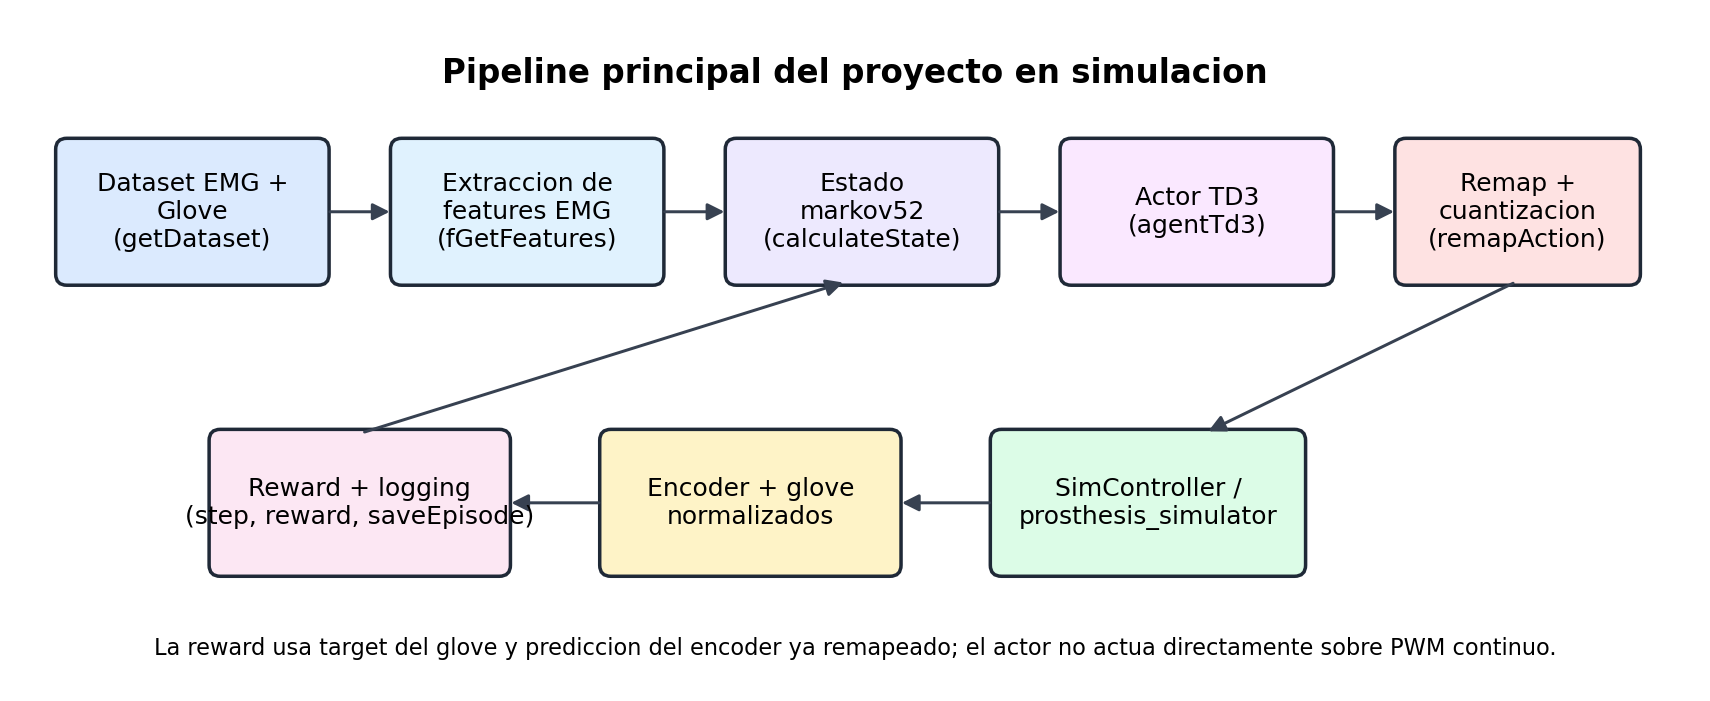
\includegraphics[width=\linewidth]{figures/guia_tecnica_pipeline_20260325.png}
\caption{Pipeline principal del proyecto en simulacion.}
\end{figure}

En ejecucion normal, el flujo es:

\begin{enumerate}
\item MATLAB entra en \texttt{trainInterface.m}.
\item \texttt{configurables()} crea el struct de configuracion activo.
\item Si hay entrenamiento nuevo, \texttt{load\_agent()} crea un TD3 desde cero.
\item Si hay evaluacion o resume training, se carga un checkpoint y se reaplican overrides mutables.
\item \texttt{Env} recibe dataset prerecorded o hardware real.
\item En cada \texttt{step}, la accion del actor se remapea a la accion efectiva del actuador.
\item El simulador o controlador aplica PWM, lee encoder y glove, reconstruye el estado y calcula la reward.
\item El entorno guarda logs detallados por paso y por episodio.
\end{enumerate}

\section{Archivos clave y para que sirve cada uno}

\begin{table}[H]
\centering
\caption{Archivos que conviene conocer primero}
\scriptsize
\setlength{\tabcolsep}{4pt}
\begin{tabularx}{\linewidth}{>{\raggedright\arraybackslash}p{3.4cm} >{\raggedright\arraybackslash}p{2.8cm} Y}
\toprule
Archivo & Tipo & Responsabilidad \\
\midrule
\makecell[tl]{\texttt{config/}\\\texttt{configurables.m}} & Configuracion & Define parametros del experimento y construye \texttt{RLtrainingOptions} o \texttt{simOpts}. \\
\makecell[tl]{\texttt{src/}\\\texttt{trainInterface.m}} & Launcher & Orquesta carga del agente, carga del dataset, creacion de entorno y ejecucion de \texttt{train} o \texttt{sim}. \\
\makecell[tl]{\texttt{agents/}\\\texttt{agentTd3.m}} & Modelo RL & Construye actor, criticos y opciones TD3. \\
\makecell[tl]{\texttt{src/@Env/}\\\texttt{calculateState.m}} & Estado & Convierte EMG y encoder a observacion \texttt{legacy44}, \texttt{markov52} o \texttt{stackedEmg132}. \\
\makecell[tl]{\texttt{src/@Env/}\\\texttt{remapActionForActuator.m}} & Accion efectiva & Aplica umbral y cuantizacion antes de enviar PWM. \\
\makecell[tl]{\texttt{src/@Env/}\\\texttt{step.m}} & Dinamica del entorno & Aplica accion, avanza tiempo, lee sensores, calcula reward y registra logs. \\
\makecell[tl]{\texttt{src/reward functions/}\\\texttt{trackingMseActionRateReward.m}} & Reward actual & Penaliza tracking MSE, magnitud de accion y cambio de accion. \\
\makecell[tl]{\texttt{src/@SimController/}\\\texttt{prosthesis\_simulator.m}} & Simulador & Genera la dinamica de la protesis. Aqui se corrigio el fallback cuando \texttt{ws} estaba vacio. \\
\makecell[tl]{\texttt{src/}\\\texttt{runCheckpointAudit.m}} & Infraestructura & Lanza auditorias reproducibles de checkpoints. \\
\makecell[tl]{\texttt{src/}\\\texttt{runCheckpointTest.m}} & Evaluacion & Ejecuta una simulacion batch sobre un checkpoint concreto. \\
\bottomrule
\end{tabularx}
\normalsize
\end{table}

\section{Lineas de codigo clave}

\subsection{\texttt{configurables.m}: configuracion global}

Estas lineas son las mas importantes para entender que experimento se esta corriendo:

\begin{lstlisting}
60: params.trainingMaxEpisodes = 12000;
61: params.trainingSaveAgentEvery = 100;
62: params.trainingPlots = "training-progress";

85: params.run_training = true;
93: params.newTraining = true;
102: params.agentFile = "";

146: params.dataset_folder = '.\data\datasets\Denis Dataset\';
150: params.comUNO = "COM4";
151: params.comGlove = "COM3";

157: params.rewardType = 'trackingMseActionRateReward';
163: params.rewardActionWeight = 0.01;
166: params.rewardDeltaActionWeight = 0.05;

180: params.speeds = 255 * [1, 1, 1, 1];
182: params.actionCommandActivationThreshold = 0.05;
183: params.actionCommandLevels = [0 64 96 128 160 192 224 255];
\end{lstlisting}

Mas abajo, el archivo cierra la definicion de observacion y runtime:

\begin{lstlisting}
265: params.observationVariant = "markov52";
267: params.stateLength = params.numEMGFeatures + 3 * numel(params.minAction);

379: params.RLtrainingOptions = rlTrainingOptions(...)
388: params.simOpts = rlSimulationOptions(...)
\end{lstlisting}

\subsection{\texttt{trainInterface.m}: donde empieza de verdad}

\begin{lstlisting}
57: if configs.newTraining
60:     observationInfo = Env.defineObservationInfo();
63:     agent = load_agent(observationInfo, actionInfo, agent_id, param_name, param_value);
65: else
67:     if strlength(string(configs.agentFile)) == 0
73:     vars = who('-file', configs.agentFile);
85:     if configs.run_training
86:         [agent, loadedAgentOverrides] = applyLoadedAgentTrainingOverrides(agent, configs);
\end{lstlisting}

Y la bifurcacion final entre entrenamiento y evaluacion es:

\begin{lstlisting}
142: if configs.run_training
144:     opts = configs.RLtrainingOptions;
148:     trainingInfo = train(agent, env, opts);
149: else
151:     simpOpts = configs.simOpts;
156:     trainingInfo = sim(agent, env, simpOpts);
\end{lstlisting}

\subsection{\texttt{agentTd3.m}: donde queda definido TD3}

\begin{lstlisting}
10: if isfield(td3, "useRecurrent") && td3.useRecurrent
13: else
14:     [actor, critics] = buildFeedforwardTd3Networks(...)
18: agentOptions = buildTd3AgentOptions(td3);
19: agent = rlTD3Agent(actor, critics, agentOptions);
\end{lstlisting}

En la configuracion valida actual, \texttt{useRecurrent = false}, asi que la ruta activa es la feedforward.

\subsection{\texttt{remapActionForActuator.m}: aqui vive la discontinuidad importante}

\begin{lstlisting}
24: if magnitude < this.actionCommandActivationThreshold
25:     continue
28: targetPwm = magnitude * maxPwm;
29: [~, idx] = min(abs(nonZeroLevels - targetPwm));
30: pwmMagnitude = nonZeroLevels(idx);
32: appliedPwm(i) = sign(actionValue) * pwmMagnitude;
33: effectiveAction(i) = appliedPwm(i) / maxPwm;
\end{lstlisting}

Esta funcion explica por que el actor no controla una planta continua pura: hay umbral y cuantizacion antes del actuador.

\subsection{\texttt{step.m}: la transicion del entorno}

\begin{lstlisting}
23: [effectiveAction, appliedPwm] = this.remapActionForActuator(action);
29: completed = this.prosthesis.sendAllSpeed(...)

46: % Advance episode time before reading the prosthesis...
48: this.episodeTic.toc(this.c);

100: [this.State, currentEncoderNorm] = this.calculateState(emg, motorData);
106: [reward, rewardVector, rewardInfo] = this.reward_function(this, effectiveAction, []);
113: this.trackingMseLog(this.c) = rewardInfo.trackingMse;
119: this.saturationFractionLog(this.c) = rewardInfo.saturationFraction;
139: if isDone && this.flagSaveTraining
140:     this.saveEpisode();
\end{lstlisting}

Las lineas 46--48 son especialmente importantes: ahi quedo corregido el desfase temporal para que la accion afecte el paso actual.

\subsection{\texttt{trackingMseActionRateReward.m}: la reward vigente}

\begin{lstlisting}
13: err = pred - target;
14: trackingMse = mean(err.^2);
16: actionL2 = mean(action.^2);
19: deltaAction = action - prevAction;
20: deltaActionL2 = mean(deltaAction.^2);
25: rewardVector = -(err.^2 + actionPenaltyVector + deltaActionPenaltyVector);
26: reward = mean(rewardVector);
35: "saturationFraction", mean(abs(action) >= 0.95)
\end{lstlisting}

La reward actual no empuja directamente por progreso o direccion, sino por error cuadratico medio y regularizacion de accion.

\subsection{\texttt{prosthesis\_simulator.m}: el bug importante ya corregido}

\begin{lstlisting}
94: ws = sim_params.(sp_txt).(dir).(m_txt).ws;
106: useCurveFallback = ws_len == 0;
108: % fit_C2.mat currently stores empty ws trajectories
110: ws = curve;
111: ws_len = curve_len;
\end{lstlisting}

Sin este fallback, el simulador podia quedarse inmovil aunque hubiese PWM no nulo. Por eso las corridas previas al fix no se consideran benchmark valido.

\section{Paths y parametros que si debes cambiar}

\subsection{Regla general}

Si trabajas en \textbf{simulacion} y mantienes la estructura actual del repo, casi todo ya esta en rutas relativas. Los cambios obligatorios aparecen solo cuando:

\begin{itemize}
\item mueves el dataset fuera del repo,
\item quieres evaluar o reanudar desde un checkpoint concreto,
\item cambias la carpeta de salida,
\item o activas hardware real.
\end{itemize}

\subsection{Tabla de paths configurables}

\scriptsize
\setlength{\tabcolsep}{4pt}
\begin{longtable}{>{\raggedright\arraybackslash}p{3.0cm} >{\raggedright\arraybackslash}p{2.6cm} >{\raggedright\arraybackslash}p{2.5cm} >{\raggedright\arraybackslash}p{5.3cm}}
\caption{Paths y parametros que conviene revisar}\\
\toprule
Parametro o ruta & Archivo y lineas & Cuando cambiarlo & Observacion practica \\
\midrule
\endfirsthead
\toprule
Parametro o ruta & Archivo y lineas & Cuando cambiarlo & Observacion practica \\
\midrule
\endhead
\makecell[tl]{\texttt{params.dataset\_}\\\texttt{folder}} & \makecell[tl]{\texttt{configurables.m:}\\\texttt{132--147}} & \makecell[tl]{Solo si el dataset\\no esta en\\\texttt{matlab\_code/data/}\\\texttt{datasets/Denis Dataset}} & En un clon limpio del repo no hace falta tocarlo. \\
\texttt{params.dataset} & \makecell[tl]{\texttt{configurables.m:}\\\texttt{135--145}} & Si quieres entrenar o evaluar con otro subconjunto de sujetos & Puede ser string unico o celda de nombres. \\
\makecell[tl]{\texttt{params.agent}\\\texttt{File}} & \makecell[tl]{\texttt{configurables.m:}\\\texttt{99--106}} & Obligatorio al evaluar o reanudar entrenamiento & Debe apuntar al \texttt{AgentXXXX.mat} deseado. Si queda vacio, \texttt{trainInterface} falla a proposito. \\
\makecell[tl]{\texttt{params.agents\_}\\\texttt{directory}} & \makecell[tl]{\texttt{configurables.m:}\\\texttt{197--200}} & Si quieres guardar resultados en otra raiz & Por defecto guarda en \makecell[tl]{\texttt{../../Agentes/}\\\texttt{trainedAgentsProtesisTest/...}}. \\
\texttt{params.comUNO} & \makecell[tl]{\texttt{configurables.m:}\\\texttt{149--151}} & Solo hardware real & Puerto serie de la protesis. No afecta simulacion. \\
\texttt{params.comGlove} & \makecell[tl]{\texttt{configurables.m:}\\\texttt{149--151}} & Solo hardware real con glove real & Puerto serie del guante. No afecta simulacion prerecorded. \\
\makecell[tl]{\texttt{agentFile} de\\\texttt{runProsthesis.m}} & \makecell[tl]{\texttt{runProsthesis.m:}\\\texttt{33--40}} & Solo si usas el script legacy de hardware & No tiene default valido. Debe ponerse a mano. \\
\makecell[tl]{\texttt{defaultCheckpoint}\\\texttt{Path()}} & \makecell[tl]{\texttt{runCheckpointTest.m:}\\\texttt{42--49}} & \makecell[tl]{Solo si llamas a\\\texttt{runCheckpoint}\\\texttt{Test()}\\sin argumentos} & Ese fallback es historico; lo correcto es pasar la ruta explicitamente. \\
\makecell[tl]{\texttt{cd(.../}\\\texttt{matlab\_code)}} & No es archivo, es requisito operativo & Siempre & Los comandos de train/test/audit asumen que MATLAB esta en \makecell[tl]{\texttt{EMG\_Prosthesis\_TD3/}\\\texttt{matlab\_code}}. \\
\end{longtable}
\normalsize

\subsection{Paths que normalmente no debes tocar}

\begin{itemize}
\item \texttt{.\textbackslash config\textbackslash normValues.mat}: ya se carga relativo en \texttt{configurables.m:209--213}.
\item \texttt{.\textbackslash src}, \texttt{.\textbackslash agents}, \texttt{.\textbackslash lib}: los \texttt{addpath} ya se resuelven desde \texttt{trainInterface.m:49--52}.
\item rutas internas de auditoria: las herramientas nuevas ya trabajan repo-relativas si se les pasa una carpeta de experimento o checkpoints explicitos.
\end{itemize}

\section{Comandos utiles}

\subsection{Sesion limpia}

\begin{lstlisting}
cd('C:/ruta/al/repo/EMG_Prosthesis_TD3/matlab_code')
clearConfigurablesOverride()
\end{lstlisting}

\subsection{Entrenamiento}

\begin{lstlisting}
cd('C:/ruta/al/repo/EMG_Prosthesis_TD3/matlab_code')
clearConfigurablesOverride()
trainInterface('td3','','')
\end{lstlisting}

\subsection{Evaluacion o test de un checkpoint}

Antes de llamar a \texttt{trainInterface}, deja en \texttt{configurables.m}:

\begin{itemize}
\item \texttt{params.run\_training = false}
\item \texttt{params.newTraining = false}
\item \texttt{params.agentFile = ".../AgentXXXX.mat"}
\end{itemize}

O bien usa el helper directo:

\begin{lstlisting}
cd('C:/ruta/al/repo/EMG_Prosthesis_TD3/matlab_code')
clearConfigurablesOverride()
trainingInfo = runCheckpointTest("C:/ruta/al/Agent7250.mat", 50, true);
\end{lstlisting}

\subsection{Auditoria de checkpoints}

\begin{lstlisting}
cd('C:/ruta/al/repo/EMG_Prosthesis_TD3/matlab_code')
clearConfigurablesOverride()
results = runCheckpointAudit(50, 200, 3, struct( ...
    'experimentDir', 'C:/ruta/a/la/corrida', ...
    'samplingPolicy', struct('mode', 'tail_every_k_last_n', 'k', 50, 'n', 12)));
\end{lstlisting}

\section{Que mirar antes de tocar codigo}

\begin{enumerate}
\item \textbf{Si cambia el comportamiento del agente}, mira primero \texttt{configurables.m}.
\item \textbf{Si el actor parece mandar cosas raras}, mira \texttt{remapActionForActuator.m}.
\item \textbf{Si el tracking deja de tener sentido}, revisa \texttt{step.m}, \texttt{calculateState.m} y la reward.
\item \textbf{Si la simulacion parece inmovil}, revisa \texttt{prosthesis\_simulator.m}.
\item \textbf{Si un checkpoint no carga bien}, revisa \texttt{trainInterface.m} y \texttt{applyLoadedAgentTrainingOverrides.m}.
\end{enumerate}

\section{Que no conviene tocar sin una razon fuerte}

\begin{itemize}
\item \texttt{observationVariant}, \texttt{rewardType} y arquitectura del agente al mismo tiempo.
\item \texttt{actionCommandActivationThreshold} y \texttt{actionCommandLevels} sin volver a auditar el efecto en control.
\item \texttt{runCheckpointTest()} sin pasar checkpoint explicito si quieres resultados reproducibles.
\item scripts legacy de hardware si el objetivo actual es simulacion.
\end{itemize}

\section{Cierre}

La idea de esta guia es que puedas abrir el repo y responder rapido cuatro preguntas:

\begin{enumerate}
\item donde arranca el flujo,
\item donde se construye el TD3,
\item donde se convierte la accion continua en accion efectiva,
\item y que rutas o parametros debes cambiar segun el escenario.
\end{enumerate}

Si se mantiene la estructura actual del repo y se trabaja en simulacion, los cambios manuales necesarios son pocos. Los dos puntos que mas se suelen tocar son \texttt{params.agentFile} y, solo si mueves datos o hardware, \texttt{dataset\_folder}, \texttt{comUNO} y \texttt{comGlove}.

\end{document}
